\subsection{SIR}

\begin{frame}
        \frametitle{Modèle SIR}

        \begin{center}
                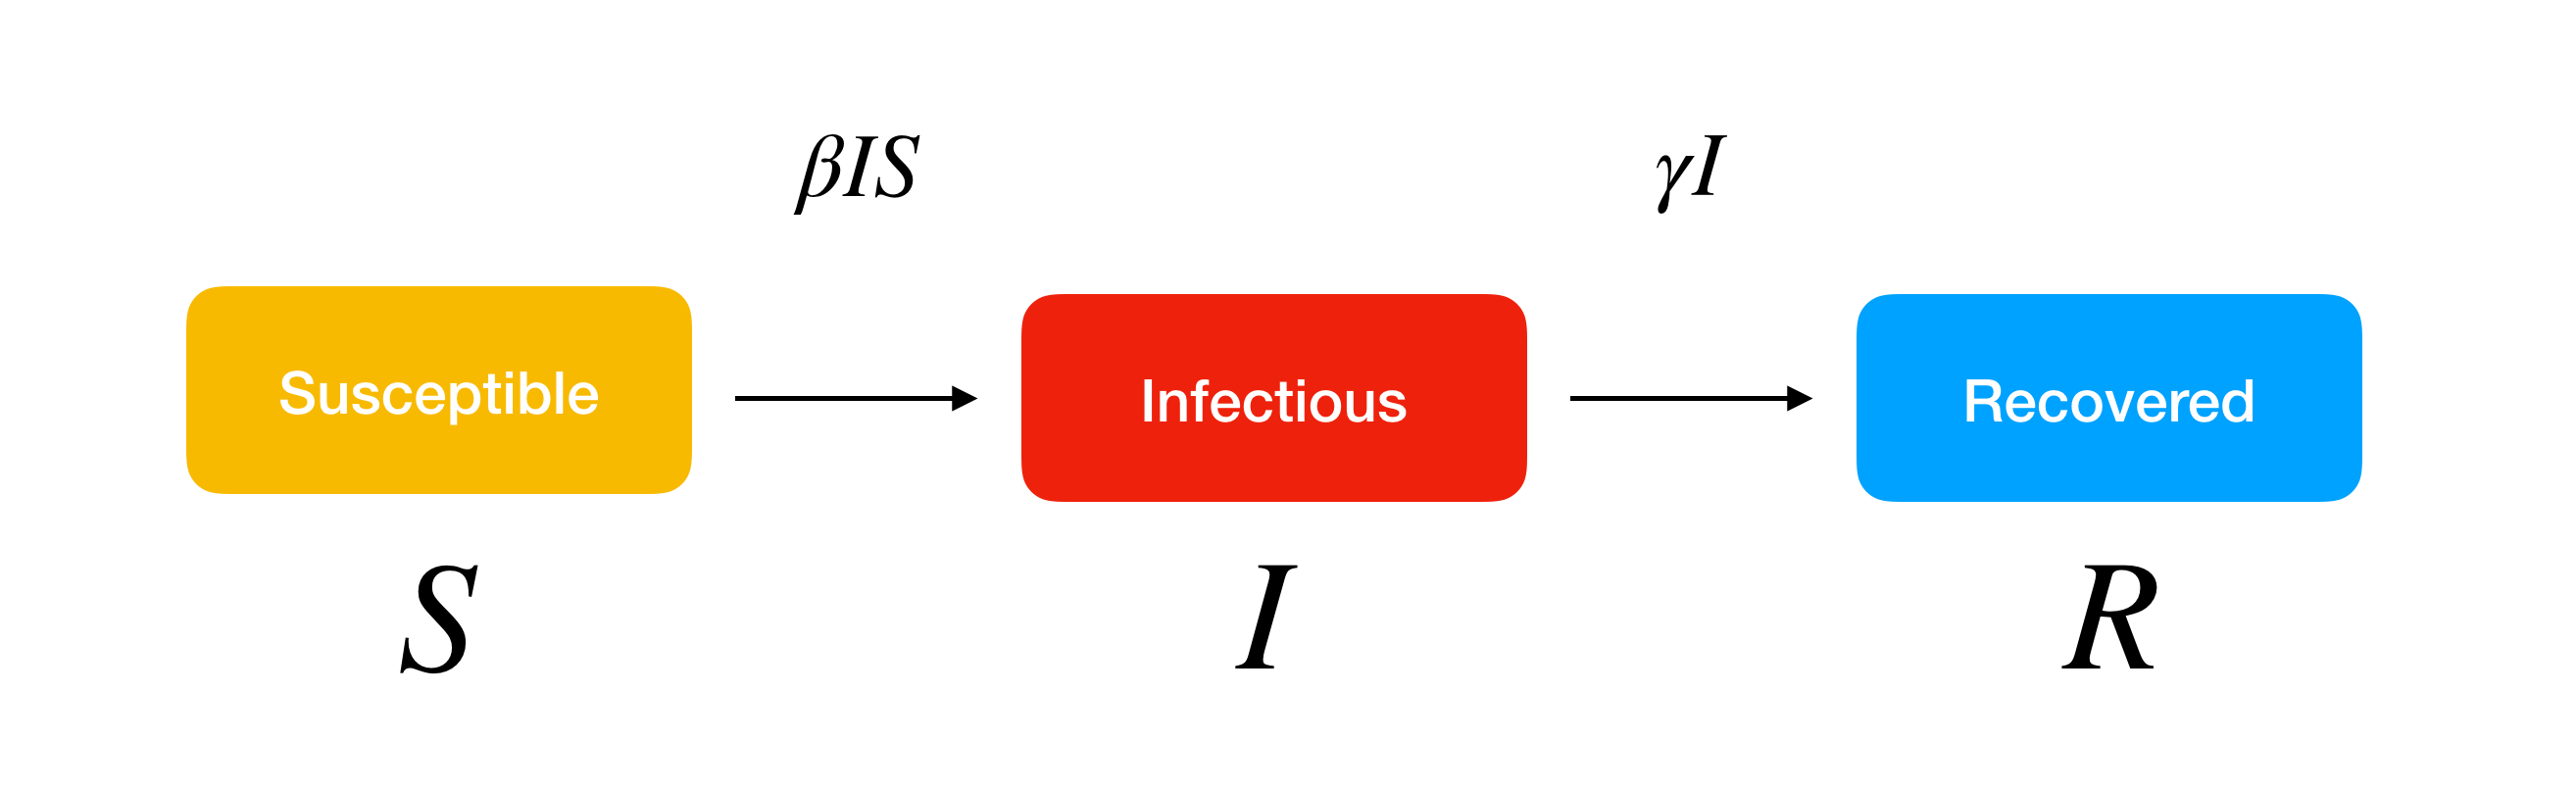
\includegraphics[width=0.75\textwidth]{sir_definition}
        \end{center}


        \begin{itemize}
                \item Susceptible - personnes saines qui n'ont pas encore contracté la maladie
                \item Infectés - les malades qui transmettent activement la maladie
                \item Rétablis - les personnes rétablies ou mortes, qui ne peuvent plus contracter la maladie.
        \end{itemize}


\end{frame}

\begin{frame}
        \frametitle{Modèle SIR}

        \begin{alertblock}{Équation}

                $$ \frac{dS}{dt} = -\frac{\beta SI}{N} \qquad \frac{dI}{dt} = \frac{\beta SI}{N} - \gamma I \qquad \frac{dR}{dt} = \gamma I $$

                \begin{itemize}
                        \item $N$ : taille totale de la population
                        \item $\beta$ : taux de contact
                        \item $\gamma$ : taux de guérison
                \end{itemize}

        \end{alertblock}
\end{frame}

\begin{frame}
        \frametitle{Modèle SIR}
			
		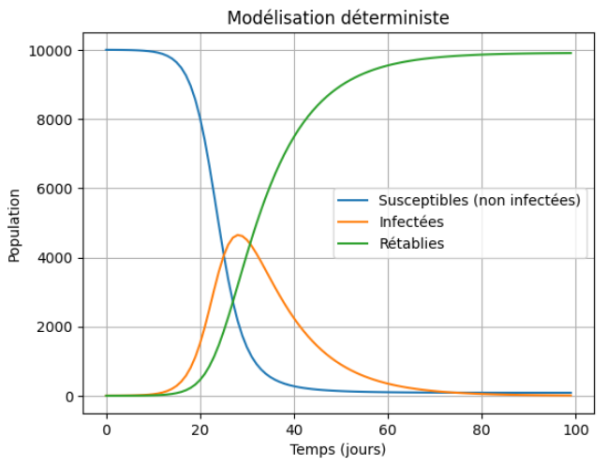
\includegraphics[width=0.50\textwidth]{sir_deterministe}
		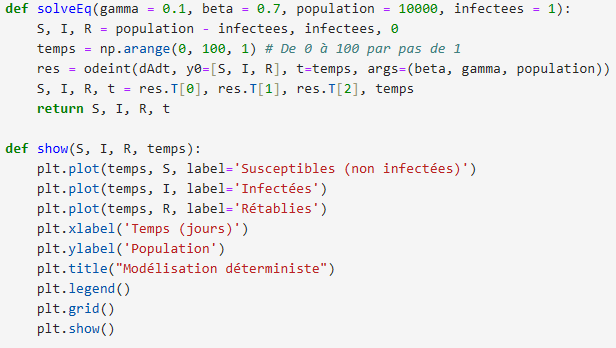
\includegraphics[width=0.50\textwidth]{sir_deterministe_python}
		
        \begin{multicols}{2}
                \begin{itemize}
                        \item $\gamma = 0.1$
                        \item $\beta = 0.48$
                        \item $N = 10000$
                        \item $I_0 = 1$
                \end{itemize}
        \end{multicols}

\end{frame}

\begin{frame}
        \frametitle{Nombre de reproduction de base ($R_0$)}

        Nombre attendu d’infection générée par un individu infectieux dans une grande population susceptible.

        \begin{alertblock}{SIR}
                $$ R_0 =  \lambda i $$
        \end{alertblock}

        \begin{itemize}
                \item $i$ : durée moyenne de la période infectieuse
                \item $\lambda$ : intensité du processus de Poisson homogène qui modélise les contacts entre les individus infectés et les individus susceptibles
        \end{itemize}
\end{frame}
